
\newenvironment{usecaseenv}{
	\def\arraystretch{2}
	\begin{tabular}{lp{11cm}}\hline
	}{
		\hline\end{tabular}
	\def\arraystretch{1}
}

\newcommand\addheading[1]{
	\multicolumn{2}{c}{\textbf{\textit{#1}}}\\ \hline
}
\newcommand\addrow[2]{\textbf{#1}\begin{minipage}[t][][t]{8cm} \end{minipage}% 
	&\begin{minipage}[t][][t]{8cm}
		#2
	\end{minipage}\\
}

% The actual command definition
\let\oldFigureName\figurename %save the old definition of the caption's figure name
\newcommand{\usecase}[8]{
	\vspace*{0.1cm} % adds a bit of padding to make it look nicer11
	\renewcommand{\figurename}{Use case} %call figure name "Use case" instead
	\begin{figure}[htbp]
		\begin{center}
			\begin{usecaseenv}
				\addrow{Description of use case:}{#2}
				\addrow{Goal of use case:}{#3}
				\addrow{Actor:}{#4}
				\addrow{Trigger:}{#5}
				\addrow{Preconditions:}{#6}
				\addrow{Steps:}{#7}
				\addrow{Expansion:}{#8}
			\end{usecaseenv}
		\end{center}
		\caption{#1}
		\label{#2}
	\end{figure}
	\renewcommand{\figurename}{\oldFigureName} %reset caption figure name
}
%% EINLEITUNG %% 
\chapter{Fundamentals}
\section{Flutter and Dart}
The framework used to develop the disease-detection application will be Flutter, which is an open-source-UI-Kit developed by Google. Flutter uses the open-source programming language Dart, which at first was designed for building Google Chrome browser-applications and later on benefited greatly from various improvements since it was released back in 2011. The programming language consequently evolved from having a lot in common with JavaScript to sharing many features with C\# and Java.
The Flutter and Dart ecosystem, which is brimming with open-source packages created by other developers from around the world, is one of the framework's best features. It enables programmers to create visually stunning applications in the shortest amount of time, by including packages from developers all over the world. Also, Dart is a client-optimized gneral-purpose programming language that supports cross-platform development. This implies that this application will be created with a single code base yet will run on both Android- and iOS-smartphones. Furthermore, the program may be launched as a web application and utilized on embedded devices. However, as part of the bachelor thesis, the development and testing process will be entirely focused on Android development. Dart is also a statically-typed language, which means that the type of each variable must be explicitly declared, making it easier to catch bugs and other issues early on in the development process. With null safety, Dart ensures that variables cannot be assigned a null value unless they are explicitly declared as nullable. This means that if a variable is expected to have a non-null value, it must be initialized with a non-null value, and any attempts to assign a null value to it will result in a compile-time error. This helps prevent null reference errors and makes it easier to write code that is safe and predictable.

 [QUELLE:DART/OVERVIEW]


%\subsection{Darts' Compiler}
%The Dart Compiler parses written code and converts it to machine code. This means that there is no way to directly run written code. [https://www.javatpoint.com/flutter-dart-programming] It's worth mentioning that Dart's compiler technology allows two distinct ways of running written code. Apps built primarily for usage on mobile devices (and desktop devices) can be compiled using the Dart VM, which supports just-in-time compilation (JIT) and ahead-of-time compilation (AOT). The JIT compilation allows the developer, in connection with Flutter, to make use of the hot reload funcionality, which decreases the time comsumption of debugging code. Dart may compile for development or production reasons when it comes to web-based projects. Its web compiler converts Dart to JavaScript. [https://dart.dev/overviewRAUTEplatform]

\subsection{Programming Paradigm}
The programming paradigm of the Dart programming language is object-oriented programming (OOP). This means that it uses objects, classes, and inheritance to organize and structure code. Dart also incorporates some functional programming concepts, such as immutable data and first-class functions, which allow for more concise and elegant code. Additionally, Dart supports asynchronous programming, which enables developers to write code that can run concurrently and handle multiple tasks at the same time. Overall, Dart's combination of OOP and functional programming paradigms makes it a versatile and powerful language for building modern web and mobile applications.

\subsection{SOLID Principals of Objectoriented Programming}
The SOLID principles are a set of guidelines for designing object-oriented software. They were introduced by Robert C. Martin in his book "Agile Software Development, Principles, Patterns, and Practices" as a way to improve the maintainability, extensibility, and flexibility of object-oriented code and to develop software that is prone to fewer bugs and has cleaner source code. [https://www.freecodecamp.org/news/solid-principles-explained-in-plain-english/]
\begin{itemize}
	\item \textbf{Single Responsibility Principle (SRP):}
	The single responsibility principle instructs the developer to develop classes and software components in such a way that they take on a maximum of one responsibility. In other words, a class should focus on a single task or piece of functionality, and should not be responsible for multiple unrelated things. This helps to reduce complexity and improve the maintainability, testability, and extensibility of a software system. Another positive side-effect of following this principle is that the written code is easier to understand and error-testing can be done more efficiently.
	
	\item \textbf{Open/Closed Principle (OCP):}
	According to the open-closed principle, software classes should be open for extension but closed for modification, which means a class should be designed in such a way that it can be easily extended or customized without changing its existing code. This allows developers to add new features or behaviors to a class without breaking its existing functionality. This suggests that these classes or software components ought to be developed in a way that allows other system entities to use their essential features without requiring access to the original entity's source code. 
	
	\item \textbf{Liskov Substitution Principle (LSP):}
	The Liskov Substitution Principle (LSP) asserts, in essence, that whenever a function uses a pointer or reference to a base object, it must also use a pointer or reference to any of its derived objects. [Software architecture with c++] One can also say, that it is an extension of the OCP. A subclass should be able to be used wherever its superclass is expected, without breaking the functionality of the program. [stickify, solid design liskov] The Liskov Substitution Principle helps to improve the flexibility and reusability of a software system.
	
	\item \textbf{Interface Segregation Principle (ISP):}
	The Interface Segregation Principle ensures that a clients of a class should not implement an interface that contains methods that are not relevant to its functionality. This helps to avoid creating large and complex interfaces that are difficult to implement and maintain. The Interface Segregation Principle promotes the creation of small, focused, and easy-to-use interfaces. 
	
	\item \textbf{Dependency Inversion Principle (DIP):}
	The key essence of the DIP is that a class should not depend on the specific implementation details of another class. Instead, it should depend on an abstract interface or a set of contracts that define how the two classes should interact.
\end{itemize}

\begin{figure}[h]
	\centering
	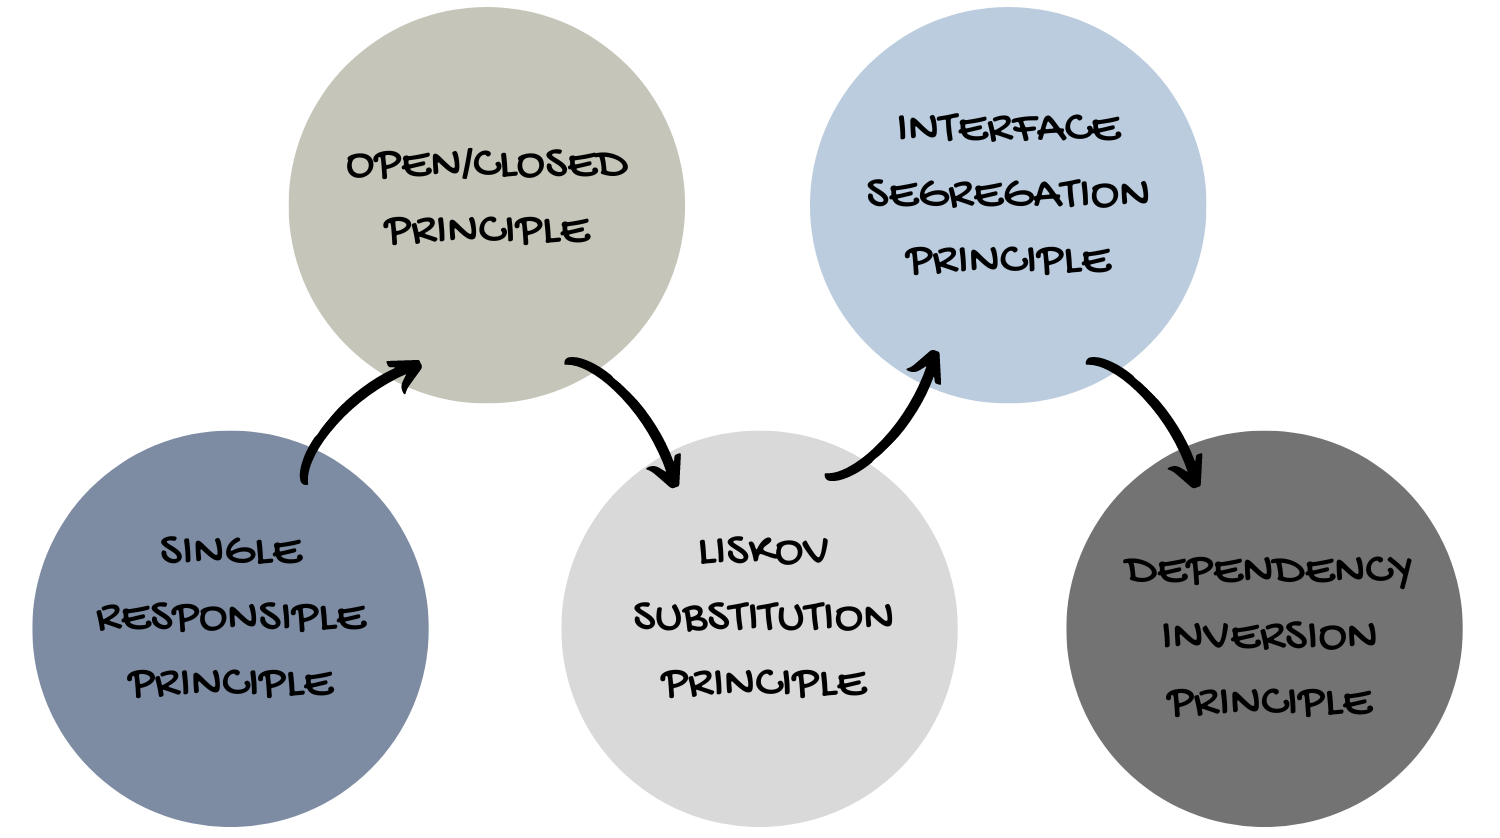
\includegraphics[scale=0.25]{solid.png}
	\caption[SOLID]{SOLID Principles}
\end{figure}
\subsection{Symptom and Disease APIs}
\subsubsection{NHS Health A to Z API}
\subsubsection{Healthwise API}
\subsubsection{ApiMedic Symptom Checker API}
